\documentclass[sigconf]{acmart}

\usepackage{subfig, amsmath, graphicx}

\acmConference[SSDBM]{SSDBM Conference}{2018}{Italy}
\acmYear{2018}
\acmDOI{xxx}
\acmISBN{xxx}
\acmArticle{x}
\acmPrice{x}

\begin{document}

\title{Size Reduction Depending on Structure Scale}

\author{Laurens Bogaardt}
\affiliation{\institution{Netherlands eScience Center}}
\email{l.bogaardt@esciencecenter.nl}

\author{Romulo Goncalves}
\affiliation{\institution{Netherlands eScience Center}}
\email{r.goncalves@esciencecenter.nl}

\author{Raul Zurita-Milla}
\affiliation{\institution{University of Twente}}
\email{r.zurita-milla@utwente.nl}

\author{Emma Izquierdo-Verdiguier}
\affiliation{\institution{University of Twente}}
\email{e.izquierdoverdiguier@utwente.nl}

\begin{abstract}
The analysis of large datasets can be time consuming and costly. Often, techniques exist to arrive at the same output, or at a close approximation, which require far less effort. This article looks at several such techniques and at the inherent scale of the structure within the data. When the values of a dataset vary slowly, e.g. in a spatial field of temperature over a country, there is a high level of autocorrelation and the structure of the field has a large scale. Datasets need not have a high resolution to describe such fields. Using generated \textit{Gaussian Random Fields} with various levels of autocorrelation, we examine rank decomposition, coarsening and approximate SVD procedures. This article outlines when certain techniques can be useful and finds a relation between performance and the scale of the structure described by the input datasets.
\end{abstract}

%\keywords{ACM proceedings, \LaTeX, text tagging}

\maketitle

\section{Introduction}
\label{sec:Introduction}

This article looks at several analysis techniques, such as the \textit{singular value decomposition} (SVD), which can be hard to apply when working with large datasets. We suggest a number of alternative implementations that may be of use when researchers have an idea about the structure scale of their data and about the desired level of accuracy. We will generate various datasets and exploit rank decomposition to analyse the data in an efficient manner. The reported results come from calculations performed in an accompanying \textit{Jupyter Notebook}~\cite{Bogaardt2018}. Note that the code was not optimised for speed, but merely serves to illustrate the procedures discussed here. The techniques discussed here are by no means novel~\cite{Golub1970, Bjorck1973, Chan1982}. However, there are domains which are less familiar analysing large datasets, so a review may be beneficial.

\subsection{Matrix Size and Rank Decomposition}
\label{sec:Introduction Matrix Size and Rank Decomposition}

Many datasets can be represented by a matrix. Take, for instance, a group of $n$ individuals who report scores on $m$ questions. Or take the temperatures at $m$ locations, measured over $n$ time periods. These values can be arranged in a matrix with $m$ rows and $n$ columns.

Like a vector, a matrix is a combination of basis vectors which indicate direction, each with a coefficient which indicates magnitude. As an extension of the vector, a matrix has two bases, the left- and the right-, or the row- and the column basis. Similarly, these bases can be changed via a rotation. Then, the coefficients will also change, leaving the resulting matrix untouched. A clever basis to rotate into is one where the basis vectors are orthonormal and each subsequent set of left- and right basis vectors explains as much of the remaining variance in the dataset as possible. Such basis vectors are called \textit{Principle Components} or \textit{Empirical Orthogonal Functions} and they may be found via an SVD of the matrix.

If a rotation can be found in which some oefficients become zero, the matrix can be described by fewer basis vectors than are available. In a sense, it is underdetermined. Its internal dimension is smaller than what would be guessed from its $m$ by $n$ size. This is the concept of matrix \textit{rank}; if the rows and columns both span a subspace of dimension~$r$, a matrix has rank~$r$. A matrix is said to have full rank if $r = \text{min}(m, n)$, the maximum number of linearly independent basis vectors. If $r < \text{min}(m, n)$, it is rank deficient.

A rank decomposition or factorization is the splitting of a matrix into a product where each factor has full rank. For example, an $m$ by $n$ matrix of rank $r$ can be decomposed it into an $m$ by $r$ matrix multiplied by an $r$ by $n$ one. Furthermore, we can choose the first factor to be an orthonormal matrix which induces a rotation, i.e. a change-of-basis. Then, the second factor captures the `action' of the matrix, written in the new bases. It is this second matrix, often smaller than the original, which is most relevant for further analyses. An SVD is a special type of rank decomposition. It results in a set of orthonormal left basis vectors $U$, a list of coefficients $s$ and a set of right basis vectors $V$. For rank deficient matrices, some of the coefficients, called singular values, will be zero.

\enlargethispage{2mm}
As noted by Martinsson, the mathematical rank $r$ of a dataset is not relevant in practice because the data originate from devices with finite precision~\cite{Martinsson2016}. Even though some singular values of a dataset are not zero, they may be small enough to be considered \textit{noise}. If we take the inherent imprecise nature of real-world data into account, we can approximate a dataset by another matrix of rank $l$, with $l < r$. Following the Eckart-Young-Mirsky theorem, the best possible approximation is one described in the same bases as the original dataset, taking a subset of the $l$ largest singular values and truncating the remainder~\cite{Eckart1936}. Taking a threshold~$\epsilon$, the dataset is said to be approximate rank deficient if some singular values fall below~$\epsilon$. Then, it has an $\epsilon$-rank of $l$ and the norm of the difference with its $l$-rank approximation is at most~$\epsilon$~\cite{Martinsson2016}.

So, we can identify three types of matrix `sizes'. The first is the size of the full matrix, $m \, n$. Storing such a dataset requires $m \, n$ units of storage and computing the product with a vector requires $m \, n$ flops. The second type is the rank decomposed version, which  requires $m \, r + r \, n$ units of storage and an equal number of flops for the vector multiplication~\cite{Martinsson2016}. If $r$ is small, this can be a substantial improvement. The final definition of `size' approximates the original dataset with a matrix of rank~$l$, resulting in even smaller storage and faster computations, while losing as little information as possible.

\subsection{Spatial Fields}
\label{sec:Introduction Spatial Fields}

In domains such a climate science and phenology, datasets are typically spatial fields, e.g. of temperature. In these fields, values vary slowly and neighbouring points are not entirely independent of one another, neither in space nor in time~\cite{Eshel2011}. Then, there is a high level of autocorrelation and the field has large scale structure. Such redundancy means the dataset is rank deficient.

To compare our techniques and to find a relation between performance and structure scale, we need to be able to generate fields which resemble those often encountered in real-world applications. In particular, we will concern ourselves with fields which combine some level of autocorrelation with some randomness. Real-valued \textit{Gaussian Random Fields} are particularly useful, as their structure scale can be captured in a single parameter, as shown in figure~\ref{fig:GaussianRandomField}. For 2D spatial fields, rotational invariance is assumed. The spectrum of such fields follows the power law described by $P(k) = c_{0} \, |\vec{k}|^{-\alpha}$ where $\vec{k}$ is the wavevector and $\alpha$ the parameter which controls the level of autocorrelation.

\vspace{-3mm}
\begin{figure}[h]
\begin{center}
\subfloat[$\alpha = 1$]{\label{fig:GaussianRandomFieldSize400Alpha1.pdf}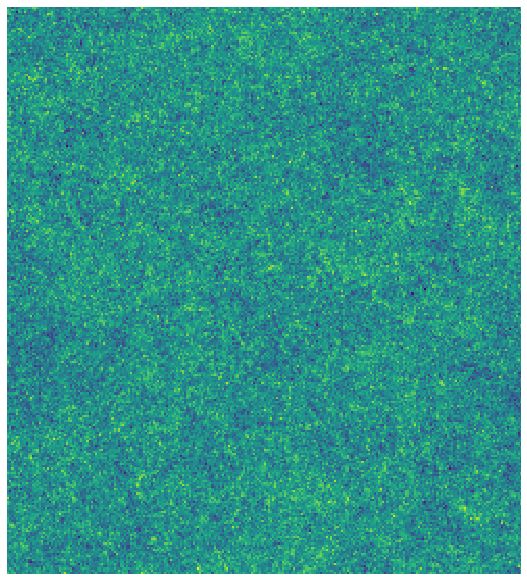
\includegraphics[scale=.31]{Results/GaussianRandomFieldSize400Alpha1.pdf}}
\hfill
\subfloat[$\alpha = 2$]{\label{fig:GaussianRandomFieldSize400Alpha2.pdf}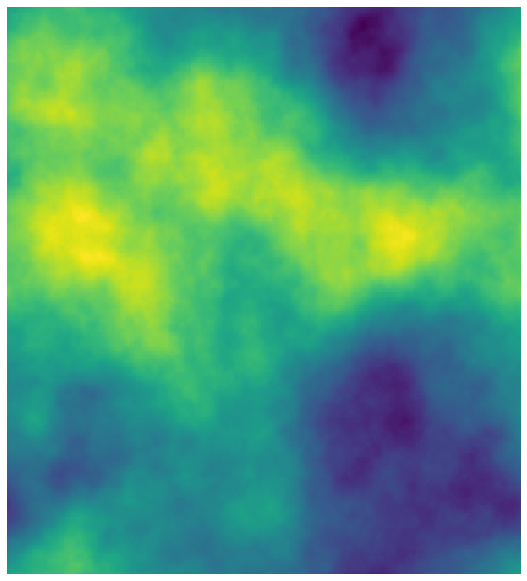
\includegraphics[scale=.31]{Results/GaussianRandomFieldSize400Alpha2.pdf}}
\hfill
\subfloat[$\alpha = 4$]{\label{fig:GaussianRandomFieldSize400Alpha4.pdf}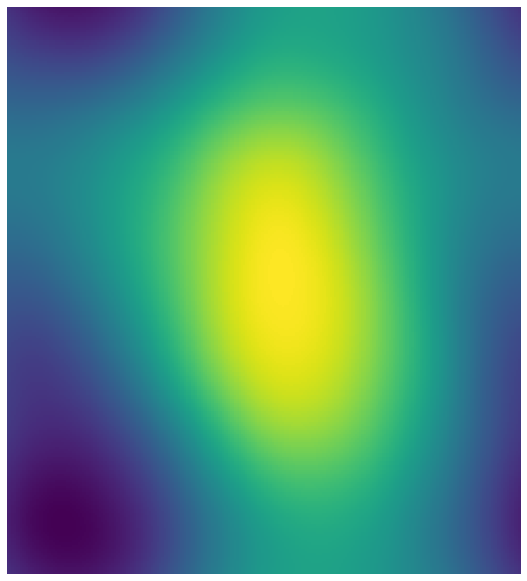
\includegraphics[scale=.31]{Results/GaussianRandomFieldSize400Alpha4.pdf}}
\caption{Gaussian Random Fields for various $\alpha$'s}
\label{fig:GaussianRandomField}
\end{center}
\end{figure}
\vspace{-3mm}

In spatial data analysis, other measures of autocorrelation are used \cite{Eshel2011, Storch1999}. These include Moran's I and the $\Gamma$ index~\cite{Moran1950, Hubert1981, PySAL}. Finally, one can devise a measure from the singular values. Each singular value indicates the amount of variance explained by its associated mode. For fields with autocorrelation, the sorted list of singular values decays quickly. One can try to fit a power law to this list and estimate the exponent, which we will call $\beta$. %While the power spectrum gives the data in terms of harmonics, an SVD gives it in terms of empirical observed functions. Therefore, the singular values will always decay more quickly than the amplitude of the wavevectors, and $\beta$ will always be larger than $\alpha$.
All these measures give an indication of the scale of the structure in the field and the level of autocorrelation in the data. Figure~\ref{fig:plotGammaAndMoransIAndBeta} plots them as a function of $\alpha$ for various generated Gaussian Random Fields.

\begin{figure}[h]
\begin{center}
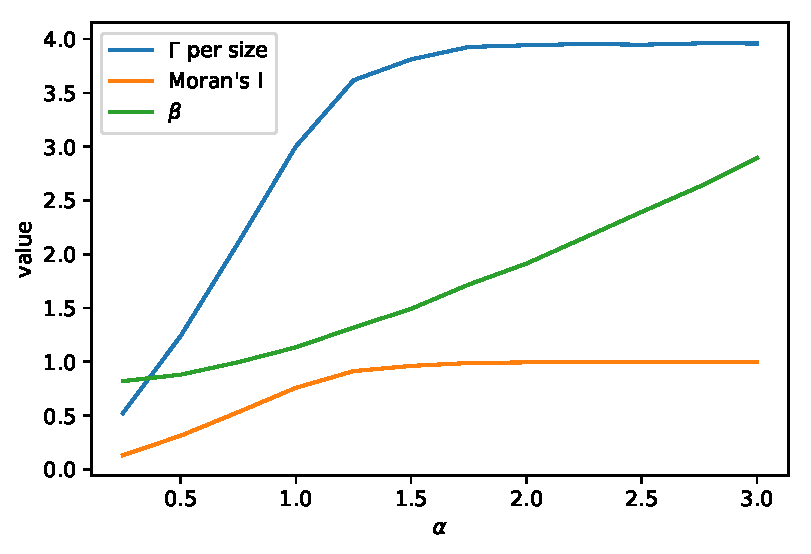
\includegraphics[width=0.8\columnwidth]{Results/plotGammaAndMoransIAndBeta.pdf}
\caption[Various measures of autocorrelation]{Measures of autocorrelation as a function of $\alpha$}
\label{fig:plotGammaAndMoransIAndBeta}
\end{center}
\end{figure}

\subsection{Spatio-Temporal Fields}
\label{sec:Introduction Spatio-Temporal Fields}

In many real-world applications, the analysis of a field does not only involve a single time period but includes data over multiple weeks, months or years. Then, we are interested in finding patterns which occur frequently. The \textit{maximum covariance analysis} (MCA) and \textit{canonical correlation analysis} (CCA) examine the cross-covariance matrix of two datasets and find patterns which occur frequently and simultaneously~\cite{Eshel2011, Storch1999}. Such a pattern, or mode, is a combination of a left- and a right basis vector. One technique to find these modes is to perform an SVD on the product of the standardised datasets. In some domains, the term SVD is used synonymously with MCA. In an MCA, modes are found where the left- and the right vector covary maximally, wereas in a CCA, they correlate maximally~\cite{Bretherton1992}.

Just as there is spatial autocorrelation, there is temporal autocorrelation, when the values of the field over the entire time period do not change drastically. In principle, there can be different levels of autocorrelation over time and over space. However, for simplicity, in this article we will use the same $\alpha$ to determine the level of autocorrelation in all dimensions.

\section{Techniques}
\label{Techniques}

This section lists four SVD related implementations to analyse large datasets by exploiting autocorrelation and rank deficiency.

\subsection{Exact Norm of Difference via SVD}
\label{sec:Techniques Exact Norm of Difference via SVD}

One often wants to find the norm of the difference between two fields. This can be done by subtracting one matrix from the other and summing the square of the elements. However, for large matrices, this may be inefficient, especially when they are rank deficient and when their SVDs are already known.

Let $|| \cdot ||$ indicate the Frobenius norm, $\left\langle \cdot \right\rangle$ the Frobenius inner product and the $\circ$ operator the Hadamard product, then the norm of the difference between matrices $A$ and $B$ is given by equation~\ref{eq:normDifferenceFromUSVs}.
\begin{equation}
\label{eq:normDifferenceFromUSVs}
\begin{split}
||A-B||^{2} & = ||A||^{2} + ||B||^{2} - 2 \left\langle A, B \right\rangle \\
& = s_{A}^{T} s_{A} + s_{B}^{T} s_{B} - 2 s_{A}^{T} \left( U_{A}^{T} U_{B} \circ V_{A}^{T} V_{B} \right) s_{B}
\end{split}
\end{equation}

Figure~\ref{fig:normDifferenceFromUSVs} shows that this procedure can determine the norm in an efficient manner, provided the number of singular values is small.
\begin{figure}[h]
\begin{center}
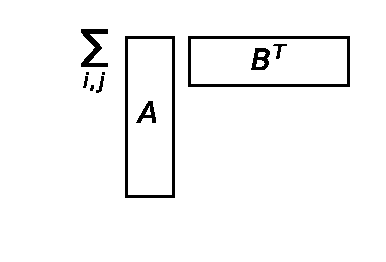
\includegraphics[width=\columnwidth]{Results/normDifferenceFromUSVs.pdf}
\caption[Exact norm of difference]{Exact norm of difference via SVD}
\label{fig:normDifferenceFromUSVs}
\end{center}
\end{figure}
%For very large datasets, the SVDs may be obtained using a random algorithm reviewed extensively in an article by Halko et al.~\cite{Halko2011}. The number of singular values will then be truncated to the $l$ largest values, similar to finding an $\epsilon$-rank approximation. In section~\ref{sec:Techniques Approximate SVD via Dimension Reduction}, we will also apply this technique to our generated fields. The resulting norm will no longer be exact, but the error can be made arbitrarily small by adjusting $l$ and $\epsilon$.

\subsection{Exact SVD via QR Decomposition}
\label{sec:Techniques Exact SVD via QR Decomposition}

In real-world applications, one often wants to find the relation between two fields. Analyses such as the MCA and CCA discussed in section~\ref{sec:Introduction Spatio-Temporal Fields} rely on performing an SVD of the cross-covariance matrix of the two fields. Take two input datasets with the various spatial gridpoints as rows and the sample of recorded values over time as columns. Centering and multiplying these gives the cross-covariance matrix. For highly rectangular matrices, when there are many spatial gridpoint but few temporal samples, the resulting cross-covaraince matrix is inefficiently large and obviously rank deficient. Performing a rank decomposition, such as the \textit{QR decomposition}, allows one to do the SVD in an efficient manner~\cite{Chan1982, Tygert2017}. As shown in figure~\ref{fig:qrProductSVD}, the result is mathematically identical to the full SVD, which means that the difference will be at machine-precision.

\begin{figure}[h]
\begin{center}
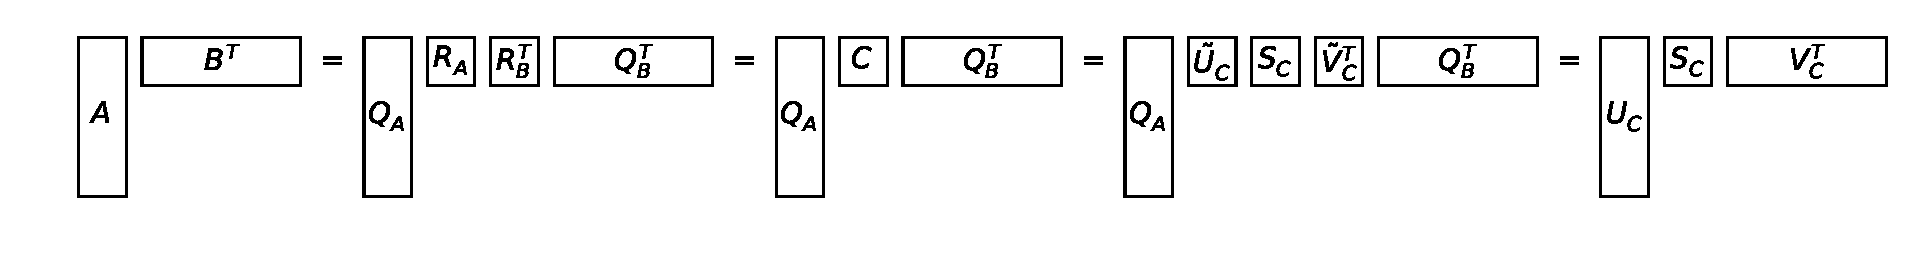
\includegraphics[width=\columnwidth]{Results/qrProductSVD.pdf}
\caption[Exact SVD via QR decomposition]{Exact SVD of a product via QR decomposition}
\label{fig:qrProductSVD}
\end{center}
\end{figure}

\subsection{Approximate SVD via Spatial Coarsening}
\label{sec:Techniques Approximate SVD via Spatial Coarsening}

Although the QR decomposition works well for two rectangular matrices, sometimes the input data is large and square. Performing an SVD on such large datasets will be time consuming. When a spatial field has large scale structure, the values of neighbouring cells do not change drastically. Perhaps these cells can be aggregated together to produce a smaller dataset which still faithfully describes the original field. In this section, we coarsen various Gaussian Random Fields by averaging patches of neighbouring gridpoints. We then compare the result with the full calculation.

\begin{figure}[h]
\begin{center}
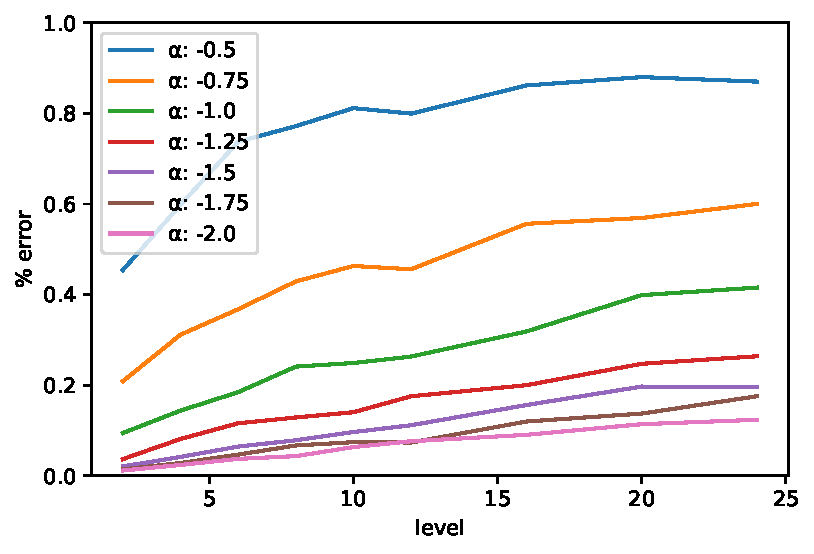
\includegraphics[width=0.8\columnwidth]{Results/plotSingleSpatialFieldViaCoarsening.pdf}
\caption[Error after coarsening a spatial field]{Error after coarsening a spatial field for various $\alpha$'s}
\label{fig:plotSingleSpatialFieldViaCoarsening}
\end{center}
\end{figure}
Figure~\ref{fig:plotSingleSpatialFieldViaCoarsening} shows the percentage error in a coarsening process for matrices of various $\alpha$'s and windows sizes of coarsening. The error is determined as the norm of the difference between the original matrix and the coarsened version, divided by the norm of the original~\cite{Bogaardt2018}. Note that a field with high autocorrelation ($\alpha=2$) differs only by a few percent from one $25$ times smaller (level $= 5$).

We can also coarsen two different fields before analysing their cross-covariance matrix. Figure~\ref{fig:plotProductSpatialTemporalFieldsViaCoarsening} shows the percentage error for various generated matrices. Due to the multiplication step in this analysis, the typical error as a result of coarsening is larger than before. As expected, the level of autocorrelation plays an important part, with larger $\alpha$'s leading to less error. The amount of error during the coarsening process will likely also depend on the similarity between the two datasets. We leave this aspect for further research.

\begin{figure}[h]
\begin{center}
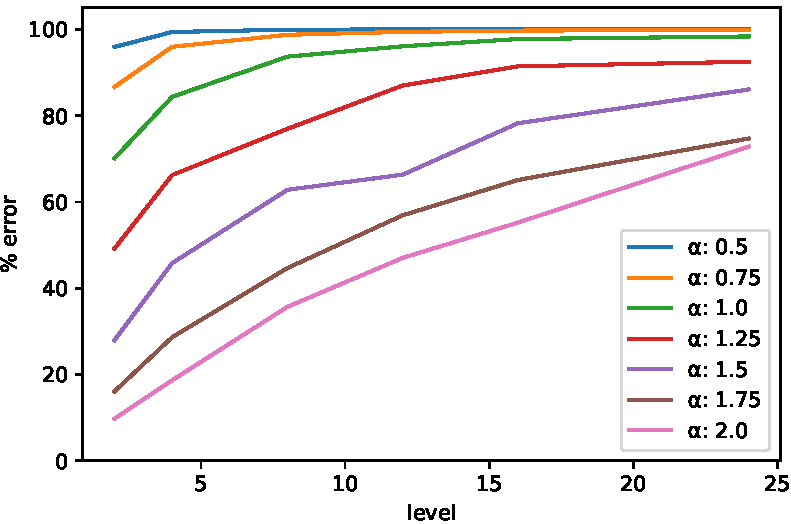
\includegraphics[width=0.8\columnwidth]{Results/plotProductSpatialTemporalFieldsViaCoarsening.pdf}
\caption[Error after coarsening product of fields]{Error after coarsening the product of two fields}
\label{fig:plotProductSpatialTemporalFieldsViaCoarsening}
\end{center}
\end{figure}
The coarsening process can speed up the calculation of the SVD, and there are additional benefits. When a target level of accuracy is set and there is an a priori estimate of the level of autocorrelation of the fields, the data collection process can be optimised. Knowing in advance at what resolution to gather data can help save time. Furthermore, in domains were satellite data is used, datasets are often not very detailed because the imaging resolution is low. Unlike local analyses of developed countries, where high resolution data is becoming more accessible, for continental or global analyses, coarse spatial resolution data may simply be the only option.

\subsection{Approx. SVD via Dimension Reduction}
\label{sec:Techniques Approximate SVD via Dimension Reduction}

The spatial coarsening process is intuitive and easy to implement. It is not, however, the most efficient way to reduce the size of a dataset. Dimension reduction refers to discarding modes which contribute little to the variance in a dataset. As mentoned in section~\ref{sec:Introduction Matrix Size and Rank Decomposition}, an SVD is precisely the procedure used to find modes which explain as much variance as possible. Discarding the smallest singular values, therefore, gives the best lower rank approximation~\cite{Eckart1936, Martinsson2016}. Performing an SVD on a large dataset, however, is computationally costly. The \textit{Randomised Dimension Reduction} process is more efficient~\cite{Halko2011, Li2016}.

As described in figure~\ref{fig:reduceSizeRandomisedSquare}, this process reduces the input matrix to a smaller square matrix of $l$ by $l$. It also gives two projection matrices which can bring the rows and columns of this smaller matrix back to the bases of the original input. It is a randomised procedure to get a $\epsilon$-rank approximation and, therefore, the error will be at the order of the size of the largest truncated singular value~\cite{Martinsson2016, Halko2011}. Our \textit{Jupyter Notebook} provides more details~\cite{Bogaardt2018}.

\begin{figure}[h]
\begin{center}
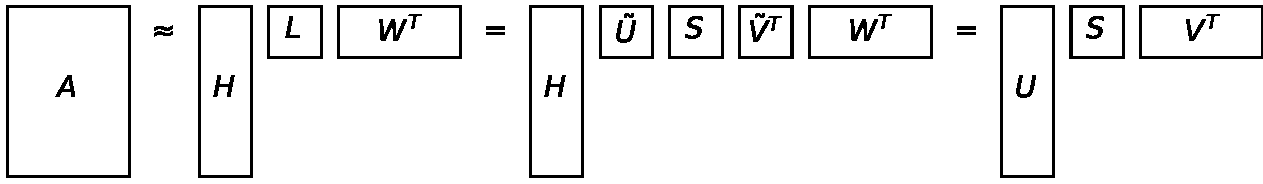
\includegraphics[width=\columnwidth]{Results/reduceSizeRandomisedSquare.pdf}
\caption[Approximate randomised SVD]{Approximate SVD via dimension reduction}
\label{fig:reduceSizeRandomisedSquare}
\end{center}
\end{figure}

%In the review article by Halko et al. on randomised dimension reduction, it is suggested to oversample the reduction. This is because the error introduced in the process is of the same order as the size of the last sampled singular value. If one is interested in the k dominant modes, reducing to a k + l, for some small l, rank approximation will ensure the first k modes are approximated quite well. Indeed, as seen below, the more modes one is interested in, the larger the difference compared with the original matrix.% quote:"the failure probability decreases superexponentially with the oversampling parameter p".
The randomised dimension reduction process can also be applied to the MCA or CCA analysis of two spatio-temporal fields. Similar to the QR product SVD, it has the advantage that the SVD is applied to a small $l$ by $l$ matrix, as seen in figure~\ref{fig:randomisedSquareProductSVD}.

\begin{figure}[h]
\begin{center}
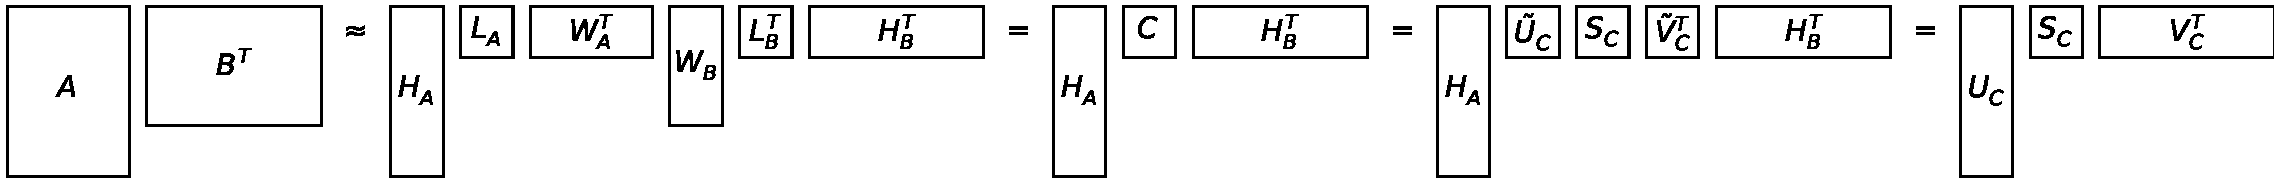
\includegraphics[width=\columnwidth]{Results/randomisedSquareProductSVD.pdf}
\caption[Approximate product SVD]{Approximate SVD for product of two fields}
\label{fig:randomisedSquareProductSVD}
\end{center}
\end{figure}

To see the effect of dimension reduction on such a matrix product, let's generate various Gaussian Random Fields and compare their cross-correlation matrix with a reduced version. Figure~\ref{fig:plotRandomisedSizeReducedMatrixProduct} shows that the results are terrible for fields with a small $\alpha$, but high levels of autocorrelation allow for substantial savings in computation time without acquiring much error.

\begin{figure}[h]
\begin{center}
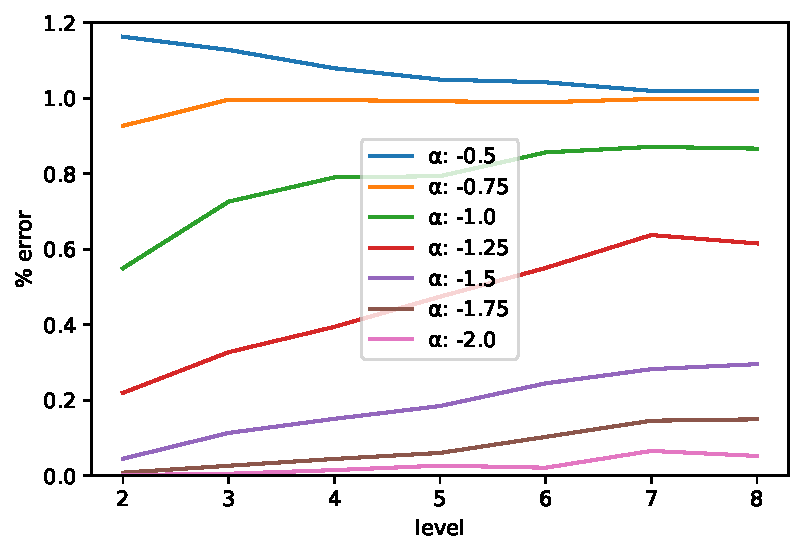
\includegraphics[width=0.8\columnwidth]{Results/plotRandomisedSizeReducedMatrixProduct.pdf}
\caption[Error after SVD]{Error after SVD of approximated fields}
\label{fig:plotRandomisedSizeReducedMatrixProduct}
\end{center}
\end{figure}

Again, we performed our analysis with two generated fields which correlated highly. Whether this correlation influences the amount of error after dimension reduction is left open.

The reduction of the number of dimensions of each input dataset is actually advised by some researchers, as a method to filter out noise~\cite{Barnett1987}. Especially when the number of temporal samples is small, outliers and random fluctuations could affect the result~\cite{Bretherton1992}. This is because any statistical analysis will choose its regression-coefficients so as to optimize the fit. It may occur that two noise-vectors in the two fields coincidentally covary and show up as dominant modes. Prefiltering can alleviate this risk.

When a dataset is too large to fit in memory, the time of transferring the matrix from storage often takes longer than the actual analysis~\cite{Halko2011}. The additional benefit of this procedure is that the randomized technique requires only a constant number of passes over the data, reducing storage communication time.

%\section{Applications}
%\label{sec:Applications}

%Phenology is the science that studies the timings of recurring biological events such as leafing and blooming as well as their causes and variations in space and time. Time series of remotely sensed images can be used to derive various land surface phenological metrics. One of these metrics is the so-called Start of Season (SOS), which indicates the beginning of photosynthetic activity in plants. In this section, we use a SOS product made for the US by processing time series of the Advanced Very High Resolution Radiometer sensor~\cite{Reed1994}. The Extended Spring Indices (SI-x) are a suite of models that transform daily temperatures into consistent phenological metrics~\cite{Schwartz2013}. We use a new long-term ($1989$ to $2014$) and high spatial resolution ($1$km) version of the Bloom index, which was recently generated for the US by adapting the SI-x models to a cloud computing environment~\cite{Izquierdo2015}. Estimated over a square subsection of the USA, we find the Bloom field to have $\alpha \approx 1.4$ and the SOS field to have $\alpha \approx 0.6$~\cite{Bogaardt2018}.

%\subsection{Approximate SVD via Spatial Coarsening}
%\label{sec:Applications Approximate SVD via Spatial Coarsening}

%After coarsening of a spatial subsection of the Bloom field for $1989$, we found an error of a few percent, in agreement with the line for $\alpha = 1.5$ on figure~\ref{fig:plotSingleSpatialFieldViaCoarsening}. For SOS, the error was slightly higher, as expected~\cite{Bogaardt2018}. After coarsening both fields for all time periods, we performed an MCA. The error was substantial, around $50\%$, but in agreement with the results of generated fields plotted in figure~\ref{fig:plotProductSpatialTemporalFieldsViaCoarsening}.

%\subsection{Approx. SVD via Dimension Reduction}
%\label{sec:Applications Approximate SVD via Dimension Reduction}

%After dimension reduction of a spatial subsection of the Bloom field for $1989$, we found a negligible error. This could be expected, as explained in the article by Halko et al.~\cite{Halko2011}. For SOS, the error was higher but still small~\cite{Bogaardt2018}. After reducing both fields for all time periods, we performed an MCA. The error was substantial, between $30\%$ and $50\%$ depending on specific parameters. These results are in agreement with those of generated fields plotted in figure~\ref{fig:plotRandomisedSizeReducedMatrixProduct}.

\section{Conclusion and Further Work}
\label{sec:Conclusion and Further Work}

Much of the analysis here relies on a priori knowledge of the level of autocorrelation. If datasets are large, it would be nice to have an algorithm to estimate Moran's I, or another measure of autocorrelation, using only a small sample of the data. It may also be interesting to extend this research to fields other than the Gaussian Random Field. This type was chosen because its structure scale can be captured in a single parameter $\alpha$. Additionally, it would be an improvement to relax the assumption that the autocorrelation in the time direction is similar to that in the spatial directions. In fact, it may even be more realistic to have different levels of autocorrelation in the North-South and in the East-West direction.

Finally, note that, unlike the coarsening procedure, the dimension reduction is not applied on each spatial field per time period, but rather on the spatially flattened timeseries. Therefore, the level of spatial autocorrelation may not be as important as the level of temporal autocorrelation. Further work can examine if better results are obtained when the dimension reduction is applied to the spatial part of the spatio-temporal fields, before it is flattened.

In conclusion, performing analyses at a coarse level can be beneficial when data collection is difficult%\footnote{In the \textit{Jupyter Notebook} accompanying this article, we applied the techniques to real datasets of phenological metrics and obtained similar results to those predicted by the Gaussian Random Fields~\cite{Bogaardt2018}.}
. Using the randomised dimension reduction can be helpful for datasets which are too large for internal memory. And, finally, rank decomposition is a useful technique of splitting datasets into square, full rank matrices together with left- and right orthonormal rotation matrices. Once the analysis is performed on the small square matrix, the output can be rotated back to the original bases, often saving computation time.

\bibliographystyle{ACM-Reference-Format}
\bibliography{Bibliography}

\end{document}
